% Figure s04f05_droplet (Session 4): lowest-Landau-level orbitals and the droplets they fill.
% The image is rendered by figures/blender/s04f05_droplet.py; the coordinates of the labels come from
% figures/blender/out/s04f05_droplet_anchors.tex. Build with figures/blender/build_figure.sh s04f05_droplet.
\documentclass[11pt,tikz,border=0pt]{standalone}
\usepackage[T1]{fontenc}
\usepackage{amsmath,amssymb,graphicx,bm}
\usepackage{xcolor}
\usetikzlibrary{arrows.meta,calc}
% The three label colors of the figures, with the same values as in src/figures_preamble.tex.
\definecolor{aqmaccent}{RGB}{31,78,121}
\definecolor{aqmbroken}{RGB}{168,42,34}
\definecolor{aqmmuted}{RGB}{125,125,125}

\newlength{\figw}\setlength{\figw}{16.14cm}   % the text width of the notes (A4, 2.7 cm margins)

\begin{document}
\begin{tikzpicture}[lbl/.style={font=\small, inner sep=1.5pt}, pnl/.style={font=\small\bfseries, inner sep=1.5pt}]
  \node[overlay, anchor=south west, inner sep=0pt] at (0,0)
    {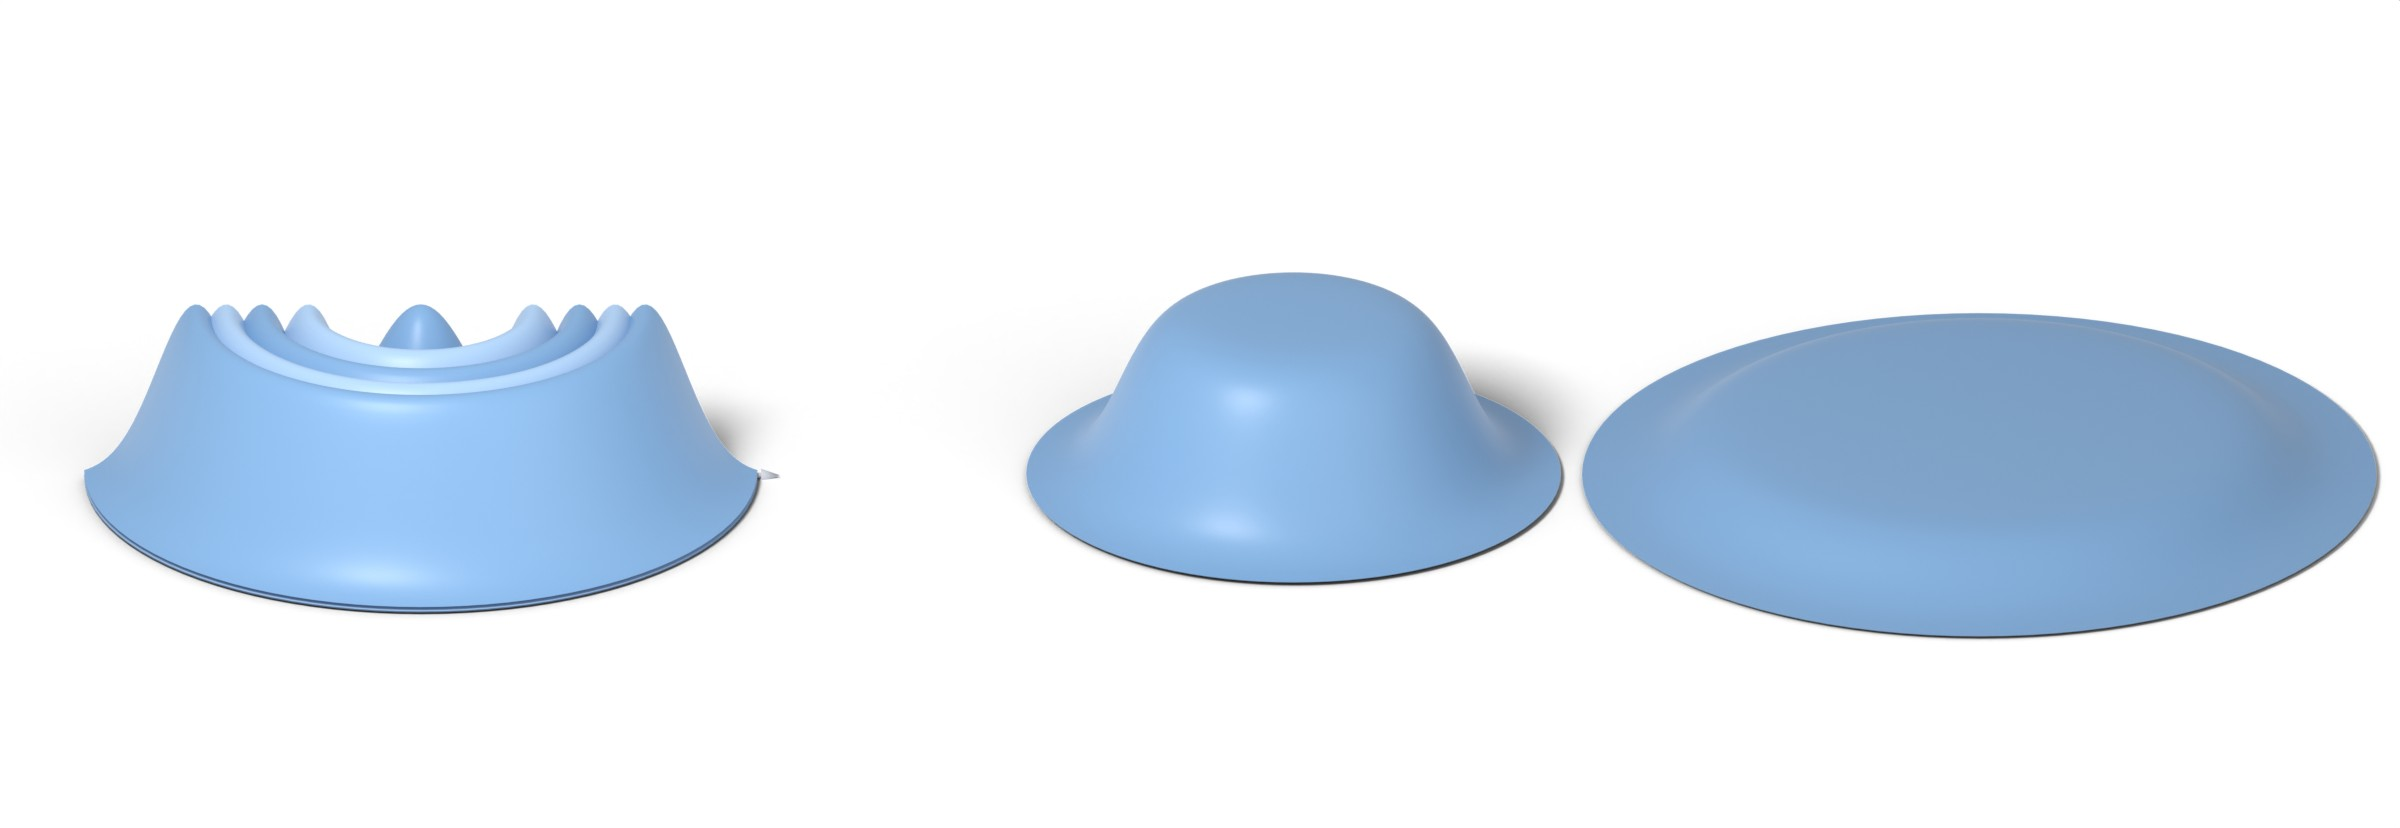
\includegraphics[width=\figw]{../blender/out/s04f05_droplet.jpg}};
  % written by build_figure.sh; the painted part of the image
\path (0.0300\figw,0.0779\figw) rectangle (0.9925\figw,0.2317\figw);

  %% written by figlib.py; x and y in units of the image width
\coordinate (m0) at (0.1753\figw,0.2241\figw);
\coordinate (m2) at (0.1286\figw,0.2241\figw);
\coordinate (m4) at (0.1092\figw,0.2241\figw);
\coordinate (m6) at (0.0943\figw,0.2241\figw);
\coordinate (m8) at (0.0818\figw,0.2241\figw);
\coordinate (ar) at (0.3249\figw,0.1470\figw);
\coordinate (apanel) at (0.0304\figw,0.2615\figw);
\coordinate (nu1) at (0.5390\figw,0.2205\figw);
\coordinate (nu3) at (0.8247\figw,0.1832\figw);
\coordinate (R1) at (0.6129\figw,0.1247\figw);
\coordinate (R3) at (0.9527\figw,0.1247\figw);
\coordinate (bpanel) at (0.4196\figw,0.2615\figw);

  \node[pnl, anchor=west] at (apanel) {(a)};
  \node[pnl, anchor=west] at (bpanel) {(b)};
  \node[lbl, anchor=south] at (m0) {$m=0$};
  \node[lbl, anchor=south] at (m8) {$m=8$};
  \node[lbl, anchor=west] at (ar) {$r$};
  \node[lbl, anchor=south, yshift=0.3cm] at (nu1) {$\nu=1$};
  \node[lbl, anchor=south, yshift=0.5cm] at (nu3) {$\nu=1/3$};
\end{tikzpicture}
\end{document}
